\newcommand{\obsvec}{\mathbf{y}}
\newcommand{\obsmat}{\mathbf{H}}
\newcommand{\obsx}{\mathbf{x}}
\newcommand{\obsxmat}{\mathbf{A}}
\newcommand{\obsdist}{\mathbf{w}}
\newcommand{\obsvar}{\mathbf{R}}

\newcommand{\statevec}{\bm{\xi}}
\newcommand{\statevar}{\mathbf{P}}
\newcommand{\statemat}{\mathbf{F}}
\newcommand{\strdist}{\mathbf{v}}
\newcommand{\strvar}{\mathbf{Q}}
\newcommand{\gain}{\mathbf{K}}
\newcommand{\statemu}{\bm{\mu}}

\newcommand{\altstrvar}{\mathbf{B}}
\newcommand{\altobsvar}{\mathbf{C}}
\newcommand{\alldist}{\bm{\varepsilon}}

\newcommand{\prederr}{\mathbf{e}}
\newcommand{\predvar}{\bm{\Sigma}}

\newcommand{\myvec}{\mbox{vec}}
\newcommand{\myvech}{\mbox{vech}}

\makeatletter
\def\pdots{\vbox{\baselineskip2.5\p@ 
  \lineskiplimit\z@ \kern2\p@\hbox{.}\hbox{.}\hbox{.}\hbox{.}}}
\makeatother

\chapter{The Kalman Filter}
\label{chap:kalman}

\section{Preamble}
\label{sec:amble}

The Kalman filter has been used ``behind the scenes'' in gretl for
quite some time, in computing ARMA estimates.  But user access to the
Kalman filter is new and it has not yet been tested to any great
extent.  We have run some tests of relatively simple cases against the
benchmark of \textsf{SsfPack Basic}.  This is state-space software
written by Koopman, Shephard and Doornik and documented in
\cite{koopman-etal99}.  It requires Doornik's \textsf{ox} program.
Both \textsf{ox} and \textsf{SsfPack} are available as free downloads
for academic use but neither is open-source; see
\url{http://www.ssfpack.com}.  Since Koopman is one of the leading
researchers in this area, presumably the results from \textsf{SsfPack}
are generally reliable.  To date we have been able to replicate the
\textsf{SsfPack} results in gretl with a high degree of precision.

We welcome both success reports and bug reports.

\section{Notation}

It seems that in econometrics everyone is happy with $y = X \beta +
u$, but we can't, as a community, make up our minds on a standard
notation for state-space models. \cite{harvey89}, \cite{hamilton94},
\cite{harvey-proietti05} and \cite{pollock99} all use different
conventions. The notation used here is based on James Hamilton's, with
slight variations.

A state-space model can be written as
%
\begin{align}
  \label{eq:state}
  \statevec_{t+1} &=  \statemat_t \statevec_t + \strdist_t \\
  \label{eq:obs}
  \obsvec_t &= \obsxmat_t'\obsx_t + \obsmat_t' \statevec_t +
  \obsdist_t 
\end{align}
%
where (\ref{eq:state}) is the state transition equation and
(\ref{eq:obs}) is the observation or measurement equation.  The state
vector, $\statevec_{t}$, is ($r \times 1$) and the vector of
observables, $\obsvec_t$, is ($n \times 1$); $\obsx_t$ is a ($k
\times 1$) vector of exogenous variables.  The ($r \times 1$) vector
$\strdist_t$ and the ($n \times 1$) vector $\obsdist_t$ are assumed to
be vector white noise:
%
\begin{align*}
E(\strdist_t \strdist_s') &= \strvar_t \mbox{ for } t = s, 
    \mbox{ otherwise } \mathbf{0} \\
E(\obsdist_t \obsdist_s') &= \obsvar_t \mbox{ for } t = s, 
    \mbox{ otherwise } \mathbf{0}
\end{align*}

The number of time-series observations will be denoted by $T$.
In the special case when $\statemat_t = \statemat$, $\obsmat_t = \obsmat$,
$\obsxmat_t = \obsxmat$, $\strvar_t = \strvar$ and $\obsvar_t =
\obsvar$, the model is said to be \emph{time-invariant}.

\subsection{The Kalman recursions}
\label{sec:kalman-recursions}

Using this notation, and assuming for the moment that $\strdist_t$ and
$\obsdist_t$ are mutually independent, the Kalman recursions can be
written as follows.

Initialization is via the unconditional mean and variance of
$\statevec_1$:
%
\begin{align*}
\hat{\statevec}_{1|0} &= E(\statevec_1) \\
\statevar_{1|0} &= E\left\{\left[\statevec_1 - E(\statevec_1)\right]
   \left[\statevec_1 - E(\statevec_1)\right]' \right\}
\end{align*}
%
Usually these are given by $\hat{\statevec}_{1|0} = \mathbf{0}$ and
%
\begin{equation}
\label{eq:inivar}
\myvec(\statevar_{1|0}) = \left[\mathbf{I}_{r^2} - \statemat \otimes
  \statemat\right]^{-1} \cdot \myvec(\strvar)
\end{equation}
but see below for further discussion of the initial variance.

Iteration then proceeds in two steps.\footnote{For a justification of
  the following formulae see the classic book by
  \cite{anderson-moore79} or, for a more modern treatment,
  \cite{pollock99} or \cite{hamilton94}.  A transcription of
  R. E. Kalman's original paper \citep{kalman60} is available at
  \url{http://www.cs.unc.edu/~welch/kalman/kalmanPaper.html}.}  First
we update the estimate of the state
%
\begin{equation}
\hat{\statevec}_{t+1|t} = \statemat_t\hat{\statevec}_{t|t-1} + 
  \gain_t \prederr_t
\end{equation}
%
where $\prederr_t$ is the prediction error for the observable:
\[
\prederr_t = \obsvec_t - \obsxmat_t'\obsx_t - \obsmat_t' \hat{\statevec}_{t|t-1}
\]
%
and $\gain_t$ is the gain matrix, given by
%
\begin{equation}
\label{eq:gain}
\gain_t = \statemat_t\statevar_{t|t-1}\obsmat_t \predvar_t^{-1}
\end{equation}
%
with
%
\[
\predvar_t = \obsmat_t'\statevar_{t|t-1}\obsmat_t + \obsvar_t
\]

The second step then updates the estimate of the variance of the state
using
%
\begin{equation}
\statevar_{t+1|t} = \statemat_t\statevar_{t|t-1}\statemat_t' -
 \gain_t \predvar_t \gain_t' + \strvar_t
\end{equation}

\subsection{Cross-correlated disturbances}

The formulation given above assumes mutual independence of the
disturbances in the state and observation equations, $\strdist_t$ and
$\obsdist_t$.  This assumption holds good in many practical
applications, but a more general formulation allows for
cross-correlation.  In place of (\ref{eq:state})--(\ref{eq:obs}) we
may write
%
\begin{align*}
  \statevec_{t+1} &= \statemat_t \statevec_t + 
     \altstrvar_t \alldist_t \\
  \obsvec_t &= \obsxmat_t'\obsx_t + \obsmat_t' \statevec_t + 
     \altobsvar_t \alldist_t 
\end{align*}
%
where $\alldist_t$ is a ($p \times 1$) disturbance vector, all the
elements of which have unit variance, $\altstrvar_t$ is ($r \times p$)
and $\altobsvar_t$ is ($n \times p$).

The no-correlation case is nested thus: define $\strdist^*_t$ and
$\obsdist^*_t$ as modified versions of $\strdist_t$ and $\obsdist_t$,
scaled such that each element has unit variance, and let
%
\[
\alldist_t =
\left[
\begin{array}{c}
  \strdist^*_t \\ \obsdist^*_t
\end{array}
\right]
\]
%
so that $p = r+n$.  Then (suppressing time subscripts for simplicity)
let 
%
\begin{align*}
  \altstrvar &= \left[
   \begin{array}{ccc} \bm{\Gamma}_{r\times r} & \pdots & 
     \mathbf{0}_{r\times n}\end{array}
  \right] \\
  \altobsvar &= \left[ 
   \begin{array}{ccc} \mathbf{0}_{n\times r} & \pdots & 
   \bm{\Lambda}_{n\times n}\end{array}
  \right]
\end{align*}
%
where $\bm{\Gamma}$ and $\bm{\Lambda}$ are lower triangular matrices
satisfying $\strvar = \bm{\Gamma} \bm{\Gamma}'$ and $\obsvar =
\bm{\Lambda} \bm{\Lambda}'$ respectively.  The zero
sub-matrices in the above expressions for $\altstrvar$ and
$\altobsvar$ produce the case of mutual independence; this corresponds
to the condition $\altstrvar \altobsvar' = \mathbf{0}$.

In the general case $p$ is not necessarily equal to $r+n$, and
$\altstrvar \altobsvar'$ may be non-zero.  This means that the
Kalman gain equation (\ref{eq:gain}) must be modified as
%
\begin{equation}
\label{eq:altgain}
\gain_t = (\statemat_t\statevar_{t|t-1}\obsmat_t + \altstrvar_t\altobsvar_t')
  \predvar_t^{-1}
\end{equation}
%
Otherwise, the equations given earlier hold good, if we write
$\altstrvar\altstrvar'$ in place of $\strvar$ and
$\altobsvar\altobsvar'$ in place of $\obsvar$.

In the account of gretl's Kalman facility below we take the
uncorrelated case as the baseline, but add remarks on how to
handle the correlated case where applicable.

\section{Intended usage}

The Kalman filter can be used in three ways: two of these are the
classic forward and backward pass, or filtering and smoothing
respectively; the third use is simulation.  In the
filtering/smoothing case you have the data $\obsvec_t$ and you want to
reconstruct the states $\statevec_t$ (and the forecast errors as a
by-product), but we may also have a computational apparatus that does
the reverse: given artificially-generated series $\obsdist_t$ and
$\strdist_t$, generate the states $\statevec_t$ (and the observables
$\obsvec_t$ as a by-product).

The usefulness of the classical filter is well known; the usefulness
of the Kalman filter as a simulation tool may be huge too. Think for
instance of Monte Carlo experiments, simulation-based inference---see
\cite{gourieroux96}---or Bayesian methods, especially in the
context of the estimation of DSGE models.

\section{Overview of syntax}

Using the Kalman filter in gretl is a two-step process.  First you set
up your filter, using a block of commands starting with
\texttt{kalman} and ending with \texttt{end kalman}---much like the
\texttt{gmm} command.  Then you invoke the functions \texttt{kfilter},
\texttt{ksmooth} or \texttt{ksimul} to do the actual work.  The next
two sections expand on these points.

\section{Defining the filter}

Each line within the \texttt{kalman} \dots{} \texttt{end kalman} block 
takes the form

\vspace{1ex}
\textsl{keyword} \textsl{value}
\vspace{1ex}

\noindent where \textsl{keyword} represents a matrix, as shown 
below. (An additional matrix which may be useful in some cases
is introduced later under the heading ``Constant term in the
state transition''.)
% % in Table~\ref{tab:keywords}.

%% \begin{table}[htbp]
\begin{center}
\begin{tabular}{lcc}
Keyword & Symbol & Dimensions \\[6pt]
\texttt{obsy}     & $\obsvec$         & $T \times n$ \\
\texttt{obsymat}  & $\obsmat$         & $r \times n$ \\
\texttt{obsx}     & $\obsx$           & $T \times k$ \\
\texttt{obsxmat}  & $\obsxmat$        & $k \times n$ \\ 
\texttt{obsvar}   & $\obsvar$         & $n \times n$ \\
\texttt{statemat} & $\statemat$       & $r \times r$ \\
\texttt{statevar} & $\strvar$         & $r \times r$ \\
\texttt{inistate} & $\hat{\statevec}_{1|0}$  & $r \times 1$ \\
\texttt{inivar}   & $\statevar_{1|0}$ & $r \times r$ \\
\end{tabular}
%% \caption{Kalman block keywords}
%% \label{tab:keywords}
\end{center}
%% \end{table}

For the data matrices $\obsvec$ and $\obsx$ the corresponding
\textsl{value} may be the name of a predefined matrix, the name of a
data series, or the name of a list of series.\footnote{Note that the
  data matrices \texttt{obsy} and \texttt{obsx} have $T$ rows.  That
  is, the column vectors $\obsvec_t$ and $\obsx_t$ in (\ref{eq:state})
  and (\ref{eq:obs}) are in fact the transposes of the $t$-dated rows
  of the full matrices.}  

For the other inputs, \textsl{value} may be the name of a predefined
matrix or, if the input in question happens to be ($1 \times $1), the
name of a scalar variable or a numerical constant.  If the
\textsl{value} of a coefficient matrix is given as the name of a
matrix or scalar variable, the input is not ``hard-wired'' into the
Kalman structure, rather a record is made of the \textit{name} of the
variable and on each run of a Kalman function (as described below) its
value is re-read.  It is therefore possible to write one
\texttt{kalman} block and then do several filtering or smoothing
passes using different sets of coefficients.\footnote{Note, however,
  that the dimensions of the various input matrices are defined via
  the initial \texttt{kalman} set-up and it is an error if any of the
  matrices are changed in size.}  An example of this technique is
provided later, in the example scripts \ref{script:armaest} and
\ref{script:loclev}.  This facility to alter the values of the
coefficients between runs of the filter is to be distinguished from
the case of \emph{time-varying} matrices, which is discussed below.

Not all of the above-mentioned inputs need be specified in every case;
some are optional. (In addition, you can specify the matrices in any
order.)  The mandatory elements are $\obsvec$, $\obsmat$, $\statemat$
and $\strvar$, so the minimal \texttt{kalman} block looks like this:

\begin{code}
kalman 
  obsy y
  obsymat H
  statemat F
  statevar Q
end kalman
\end{code} 

The optional matrices are listed below, along with the implication
of omitting the given matrix.

\begin{center}
\begin{tabular}{ll}
Keyword & If omitted\dots \\ [6pt]
\texttt{obsx} & no exogenous variables in observation equation\\
\texttt{obsxmat} & no exogenous variables in observation equation\\
\texttt{obsvar} & no disturbance term in observation equation\\
\texttt{inistate} & $\hat{\statevec}_{1|0}$ is set to a zero vector\\
\texttt{inivar} & $\statevar_{1|0}$ is set automatically\\
\end{tabular}
\end{center}

It might appear that the \texttt{obsx} ($\obsx$) and \texttt{obsxmat}
($\obsxmat$) matrices must go together---either both are given or
neither is given.  But an exception is granted for convenience.  If
the observation equation includes a constant but no additional
exogenous variables, you can give a ($1 \times n$) value for
$\obsxmat$ without having to specify \texttt{obsx}.  More generally,
if the row dimension of $\obsxmat$ is 1 greater than the column
dimension of $\obsx$, it is assumed that the first element of
$\obsxmat$ is associated with an implicit column of 1s.

Regarding the automatic initialization of $\statevar_{1|0}$ (in case
no \texttt{inivar} input is given): by default this is done as in
equation (\ref{eq:inivar}).  However, this method is applicable only
if all the eigenvalues of $\statemat$ lie inside the unit circle.  If
this condition is not satisfied we instead apply a diffuse prior,
setting $\statevar_{1|0} = \kappa \mathbf{I}_r$ with $\kappa = 10^7$.
If you wish to impose this diffuse prior from the outset, append the
option flag \verb|--diffuse| to the \texttt{end kalman}
statement.\footnote{ Initialization of the Kalman filter outside of
  the case where equation (\ref{eq:inivar}) applies has been the
  subject of much discussion in the literature---see for example
  \cite{dejong91}, \cite{koopman97}.  At present gretl does not
  implement any of the more elaborate proposals that have been made.}

\subsection{Time-varying matrices}

Any or all of the matrices \texttt{obsymat}, \texttt{obsxmat},
\texttt{obsvar}, \texttt{statemat} and \texttt{statevar} may be
time-varying.  In that case the \textsl{value} corresponding to the
matrix keyword should be given in a special form: the name of an
existing matrix plus a function call which modifies that matrix,
separated by a semicolon.  Note that in this case you must use
a matrix variable, even if the matrix in question happens to be
$1 \times 1$. 

For example, suppose the matrix $\obsmat$ is time-varying.  Then we
might write
%
\begin{code}
obsymat H ; modify_H(&H, theta)
\end{code}
%
where \texttt{modify\_H} is a user-defined function which modifies
matrix \texttt{H} (and \texttt{theta} is a suitable additional
argument to that function, if required).

The above is just an illustration: the matrix argument does not have
to come first, and the function can have as many arguments as you
like.  The essential point is that the function must modify the
specified matrix, which requires that it be given as an argument in
``pointer'' form (preceded by \verb|&|).  The function need not return
any value directly; if it does, that value is ignored.

Such matrix-modifying functions will be called at each time-step of
the filter operation, prior to performing any calculations.  They have
access to the current time-step of the Kalman filter via the internal
variable \verb+$kalman_t+, which has value 1 on the first step, 2 on
the second, and so on, up to step $T$.  They also have access to the
previous $n$-vector of forecast errors, $\prederr_{t-1}$, under the
name \verb+$kalman_uhat+.  When $t=1$ this will be a zero vector.

\subsection{Correlated disturbances}

Defining a filter in which the disturbances $\strdist_t$ and
$\obsdist_t$ are correlated involves one modification to the account
given above.  If you append the \verb|--cross| option flag to the
\texttt{end kalman} statement, then the matrices corresponding to
the keywords \texttt{statevar} and \texttt{obsvar} are interpreted
not as $\strvar$ and $\obsvar$ but rather as $\altstrvar$ and
$\altobsvar$ as discussed in section~\ref{sec:kalman-recursions}.
Gretl then computes $\strvar = \altstrvar\altstrvar'$ and
$\obsvar = \altobsvar\altobsvar'$ as well as the cross-product
$\altstrvar\altobsvar'$ and utilizes the modified expression for
the gain as given in equation (\ref{eq:altgain}).  As mentioned
above, $\altstrvar$ should be ($r \times p$) and $\altobsvar$
should be ($n \times p$), where $p$ is the number of elements
in the combined disturbance vector $\alldist_t$.

\subsection{Constant term in the state transition}

In some applications it is useful to be able to represent a constant
term in the state transition equation explicitly; that is, equation
(\ref{eq:state}) becomes
%
\begin{equation}
\label{eq:statemu}
\statevec_{t+1} =  \statemu + \statemat_t \statevec_t + \strdist_t
\end{equation}
%
This is never strictly necessary; the system (\ref{eq:state}) and
(\ref{eq:obs}) is general enough to accommodate such a term, by
absorbing it as an extra (unvarying) element in the state vector. But
this comes at the cost of expanding all the matrices that touch the
state ($\statevec$, $\statemat$, $\strdist$, $\strvar$, $\obsmat$),
making the model relatively awkward to formulate and forecasts
relatively expensive to compute.

As a simple illustration, consider a univariate model in which the
state, $s_t$, is just a random walk with drift $\mu$ and the observed
variable, $y_t$, is the state plus white noise:
\begin{align}
  \label{eq:state-rw}
  s_{t+1} &=  \mu + s_t + v_t \\
  \label{eq:obs-y}
  y_t &= s_t + w_t 
\end{align}
%
Putting this into the standard form of (\ref{eq:state}) and
(\ref{eq:obs}) we get:
%
\begin{align*}
\left[ \begin{array}{c} s_{t+1} \\ \mu \end{array} \right] 
&=
\left[ \begin{array}{cc} 1 & 1 \\ 0 & 1 \end{array} \right]
\left[ \begin{array}{c} s_t \\ \mu \end{array} \right] +
\left[ \begin{array}{c} v_t \\ 0 \end{array} \right] ,
\qquad
\strvar = \left[ 
\begin{array}{cc} \sigma^2_v & 0 \\ 0 & 0 \end{array} 
\right] \\
y_t &= 
\left[ \begin{array}{cc} 1 & 0 \end{array} \right]
\left[ \begin{array}{c} s_t \\ \mu \end{array} \right] + w_t
\end{align*}

In such a simple case the notational and computational burden is not
very great; nonetheless it is clearly more ``natural'' to express this
system in the form of (\ref{eq:state-rw}) and (\ref{eq:obs-y}) and in
a multivariate model the gain in parsimony could be substantial.

For this reason we support the use of an additional named matrix
in the \texttt{kalman} setup, namely \texttt{stconst}. This
corresponds to $\statemu$ in equation (\ref{eq:statemu}); it
should be an $r \times 1$ vector (or if $r=1$ may be given as
the name of a scalar variable). The use of \texttt{stconst}
in setting up a filter corresponding to (\ref{eq:state-rw}) and
(\ref{eq:obs-y}) is shown below.


\begin{code}
matrix H = {1}
matrix R = {1}
matrix F = {1}
matrix Q = {1}
matrix mu = {0.05}

kalman 
  obsy y
  obsymat H
  obsvar R
  statemat F
  statevar Q
  stconst mu
end kalman
\end{code} 

\subsection{Handling of missing values}

It is acceptable for the data matrices, \texttt{obsy} and
\texttt{obsx}, to contain missing values.  In this case the filtering
operation will work around the missing values, and the \texttt{ksmooth}
function can be used to obtain estimates of these values.  However,
there are two points to note.

First, gretl's default behavior is to skip missing observations when
constructing matrices from data series.  To change this, use the \texttt{set} 
command thus:
%
\begin{code}
set skip_missing off
\end{code}

Second, the handling of missing values is not yet quite right for the
case where the observable vector $\obsvec_t$ contains more than one
element.  At present, if any of the elements of $\obsvec_t$ are
missing the entire observation is ignored.  Clearly it should be
possible to make use of any non-missing elements, and this is not
very difficult in principle, it's just awkward and is not
implemented yet.

\subsection{Persistence and identity of the filter}

At present there is no facility to create a ``named filter''.  Only
one filter can exist at any point in time, namely the one created by
the last \texttt{kalman} block.\footnote{This is not quite true: more
  precisely, there can be no more than one Kalman filter \textit{at
    each level of function execution}.  That is, if a gretl script
  creates a Kalman filter, a user-defined function called from that
  script may also create a filter, without interfering with the
  original one.}  If a filter is already defined, and you give a new
\texttt{kalman} block, the old filter is over-written.  Otherwise the
existing filter persists (and remains available for the
\texttt{kfilter}, \texttt{ksmooth} and \texttt{ksimul} functions)
until either (a) the gretl session is terminated or (b) the command
\texttt{delete kalman} is given.


\section{The \texttt{kfilter} function}

Once a filter is established, as discussed in the previous section,
\texttt{kfilter} can be used to run a forward, forecasting pass.
This function returns a scalar code: 0 for successful completion, or 1
if numerical problems were encountered.  On successful completion, two
scalar accessor variables become available: \verb+$kalman_lnl+, which
gives the overall log-likelihood under the joint normality assumption,
%
\[
  \ell = -\frac{1}{2} \left[nT \log(2 \pi) + \sum_{t=1}^T\log \left|\predvar_t\right| + 
    \sum_{t=1}^T\prederr_t'\predvar_t^{-1} \prederr_t
  \right]
\]
%
and \verb+$kalman_s2+, which gives the estimated variance,
%
\[
\hat{\sigma}^2 = \frac{1}{nT} 
   \sum_{t=1}^T\prederr_t'\predvar_t^{-1} \prederr_t
\]
(but see below for modifications to these formulae for the case of a
diffuse prior).  In addition the accessor \verb+$kalman_llt+ gives a
($T \times 1$) vector, element $t$ of which is
%
\[
  \ell_t = -\frac{1}{2} \left[n \log(2 \pi) + \log \left|\predvar_t\right| + 
    \prederr_t'\predvar_t^{-1} \prederr_t
  \right]
\]
%

The \texttt{kfilter} function does not require any arguments, but up
to five matrix quantities may be retrieved via optional pointer
arguments.  Each of these matrices has $T$ rows, one for each
time-step; the contents of the rows are shown in the following
listing.
%
\begin{enumerate}
\item Forecast errors for the observable variables: $\prederr_t'$, $n$
  columns.
\item Variance matrix for the forecast errors: $\myvech(\predvar_t)'$,
  $n(n+1)/2$ columns.
\item Estimate of the state vector: $\hat{\statevec}_{t|t-1}'$, $r$ columns.
\item MSE of estimate of the state vector:
  $\myvech(\statevar_{t|t-1})'$, $r(r+1)/2$ columns.
\item Kalman gain: $\myvec(\gain_t)'$, $rn$ columns.
\end{enumerate}

Unwanted trailing arguments can be omitted, otherwise unwanted
arguments can be skipped by using the keyword \texttt{null}.  For
example, the following call retrieves the forecast errors in the
matrix \texttt{E} and the estimate of the state vector in \texttt{S}:
%
\begin{code}
matrix E S
kfilter(&E, null, &S)
\end{code}

Matrices given as pointer arguments do not have to be correctly
dimensioned in advance; they will be resized to receive the specified
content.

Further note: in general, the arguments to \texttt{kfilter} should all
be matrix-pointers, but under two conditions you can give a pointer to
a series variable instead.  The conditions are: (i) the matrix in
question has just one column in context (for example, the first two
matrices will have a single column if the length of the observables
vector, $n$, equals 1) and (ii) the time-series length of the filter
is equal to the current gretl sample size.

\subsection{Likelihood under the diffuse prior}

There seems to be general agreement in the literature that the
log-likelihood calculation should be modified in the case of a diffuse
prior for $\statevar_{1|0}$.  However, it is not clear to us that
there is a well-defined ``correct'' method for this.  At present we
emulate \textsf{SsfPack} (see \cite{koopman-etal99} and
section~\ref{sec:amble}).  In case $\statevar_{1|0} = \kappa
\mathbf{I}_r$, we set $d = r$ and calculate
%
\[
  \ell = -\frac{1}{2} \left[(nT-d) \log(2 \pi) + 
    \sum_{t=1}^T\log \left|\predvar_t\right| + 
    \sum_{t=1}^T\prederr_t'\predvar_t^{-1} \prederr_t
    - d \log(\kappa)
  \right]
\]
%
and
%
\[
\hat{\sigma}^2 = \frac{1}{nT-d} 
   \sum_{t=1}^T\prederr_t'\predvar_t^{-1} \prederr_t
\]

\section{The \texttt{ksmooth} function}

This function returns the ($T \times r$) matrix of smoothed estimates
of the state vector---that is, estimates based on all $T$
observations: row $t$ of this matrix holds $\hat{\statevec}_{t|T}'$.  This
function has no required arguments but it offers one optional
matrix-pointer argument, which retrieves the variance of the smoothed
state estimate, $\statevar_{t|T}$.  The latter matrix is ($T \times
r(r+1)/2$); each row is in transposed vech form.  Examples:
%
\begin{code}
matrix S = ksmooth()  # smoothed state only
matrix P
S = ksmooth(&P)       # the variance is wanted
\end{code}

These values are computed via a backward pass of the filter, from
$t = T$ to $t = 1$, as follows:
%
\begin{align*}
\mathbf{L}_t &= \statemat_t - \gain_t \obsmat_t' \\
\mathbf{u}_{t-1} &= \obsmat_t \predvar_t^{-1} \prederr_t 
 + \mathbf{L}_t' \mathbf{u}_t \\
\mathbf{U}_{t-1} &= \obsmat_t \predvar_t^{-1} \obsmat_t' + 
  \mathbf{L}_t' \mathbf{U}_t \mathbf{L}_t \\
\hat{\statevec}_{t|T} &= \hat{\statevec}_{t|t-1} + 
  \statevar_{t|t-1} \mathbf{u}_{t-1} \\
\statevar_{t|T} &= \statevar_{t|t-1} - 
  \statevar_{t|t-1} \mathbf{U}_{t-1} \statevar_{t|t-1}
\end{align*}
%
with initial values $\mathbf{u}_T = 0$ and $\mathbf{U}_T =
0$.\footnote{See I. Karibzhanov's exposition at
\url{http://www.econ.umn.edu/~karib003/help/kalcvs.htm}.}

This iteration is preceded by a special forward pass in which the
matrices $\gain_t$, $\predvar_t^{-1}$, $\hat{\statevec}_{t|t-1}$ and
$\statevar_{t|t-1}$ are stored for all $t$.  If $\statemat$
is time-varying, its values for all $t$ are stored on the forward
pass, and similarly for $\obsmat$.


\section{The \texttt{ksimul} function}

This simulation function takes up to three arguments.  The first,
mandatory, argument is a ($T \times r$) matrix containing artificial
disturbances for the state transition equation: row $t$ of this matrix
represents $\strdist_t'$.  If the current filter has a non-null
$\obsvar$ (\texttt{obsvar}) matrix, then the second argument should be
a ($T \times n$) matrix containing artificial disturbances for the
observation equation, on the same pattern.  Otherwise the second
argument should be given as \texttt{null}.  If $r=1$ you may give a
series for the first argument, and if $n=1$ a series is acceptable for
the second argument.

Provided that the current filter does not include exogenous variables
in the observation equation (\texttt{obsx}), the $T$ for simulation
need not equal that defined by the original \texttt{obsy} data matrix:
in effect $T$ is temporarily redefined by the row dimension of the
first argument to \texttt{ksimul}.  Once the simulation is completed,
the $T$ value associated with the original data is restored.

The value returned by \texttt{ksimul} is a ($T \times n$) matrix
holding simulated values for the observables at each time step.  A
third optional matrix-pointer argument allows you to retrieve a ($T
\times r$) matrix holding the simulated state vector.  Examples:
%
\begin{code}
matrix Y = ksimul(V)    # obsvar is null
Y = ksimul(V, W)        # obsvar is non-null
matrix S
Y = ksimul(V, null, &S) # the simulated state is wanted
\end{code}

The initial value $\statevec_1$ is calculated thus: we find the matrix
$\mathbf{T}$ such that $\mathbf{T}\mathbf{T}' = \statevar_{1|0}$ (as
given by the \texttt{inivar} element in the \texttt{kalman} block),
multiply it into $\strdist_1$, and add the result to $\statevec_{1|0}$
(as given by \texttt{inistate}).

If the disturbances are correlated across the two equations the
arguments to \texttt{ksimul} must be revised: the first argument
should be a ($T \times p$) matrix, each row of which represents
$\alldist_t'$ (see section~\ref{sec:kalman-recursions}), and the
second argument should be given as \texttt{null}.



\section{Example 1: ARMA estimation}
\label{sec:example_arma}

As is well known, the Kalman filter provides a very efficient way to
compute the likelihood of ARMA models; as an example, take an
ARMA(1,1) model
\[
  y_t = \phi y_{t-1} + \varepsilon_t + \theta \varepsilon_{t-1}
\]
One of the ways the above equation can be cast in state-space form is
by defining a latent process $\xi_t = (1 - \phi L)^{-1}
\varepsilon_t$.   The observation equation corresponding to (\ref{eq:obs})
is then
%
\begin{equation}
y_t = \xi_t + \theta \xi_{t-1} \label{eq:arma-meas}
\end{equation}
%
and the state transition equation corresponding to (\ref{eq:state}) is
%
\[
  \left[ \begin{array}{c} \xi_t \\ \xi_{t-1} \end{array} \right] =
  \left[ \begin{array}{cc} \phi & 0 \\ 1 & 0 \end{array} \right]
  \left[ \begin{array}{c} \xi_{t-1} \\ \xi_{t-2} \end{array} \right] +
  \left[ \begin{array}{c} \varepsilon_t \\ 0 \end{array} \right] 
\]

The gretl syntax for a corresponding \texttt{kalman} block would be
\begin{code}
matrix H = {1; theta}
matrix F = {phi, 0; 1, 0}
matrix Q = {s^2, 0; 0, 0}

kalman
    obsy y
    obsymat H
    statemat F
    statevar Q
end kalman
\end{code}
Note that the observation equation (\ref{eq:arma-meas}) does not
include an ``error term''; this is equivalent to saying that
$V(\obsdist_t) = 0$ and, as a consequence, the \texttt{kalman} block
does not include an \texttt{obsvar} keyword.

Once the filter is set up, all it takes to compute the log-likelihood
for given values of $\phi$, $\theta$ and $\sigma^2$ is to execute the
\texttt{kfilter()} function and use the \verb+$kalman_lnl+ accessor
(which returns the total log-likelihood) or, more appropriately if the
likelihood has to be maximized through \texttt{mle}, the
\verb+$kalman_llt+ accessor, which returns the series of individual
contribution to the log-likelihood for each observation. An example
is shown in script~\ref{script:armaest}.

\begin{script}[htbp]
  \caption{ARMA estimation}
  \label{script:armaest}
\begin{scode}
function void arma11_via_kalman(series y)
    /* parameter initalization */
    phi = 0
    theta = 0
    sigma = 1

    /* Kalman filter setup */
    matrix H = {1; theta}
    matrix F = {phi, 0; 1, 0}
    matrix Q = {sigma^2, 0; 0, 0}

    kalman
        obsy y
        obsymat H
        statemat F
        statevar Q
    end kalman

    /* maximum likelihood estimation */
    mle logl = ERR ? NA : $kalman_llt
        H[2] = theta
        F[1,1] = phi
        Q[1,1] = sigma^2
        ERR = kfilter()
        params phi theta sigma
    end mle -h
end function

# ------------------------ main ---------------------------

open arma.gdt        # open the "arma" example dataset
arma11_via_kalman(y) # estimate an arma(1,1) model
arma 1 1 ; y --nc    # check via native command
\end{scode}
\end{script}

\section{Example 2: local level model}
\label{sec:example_loclev}

Suppose we have a series $y_t = \mu_t + \varepsilon_t$, where $\mu_t$
is a random walk with normal increments of variance $\sigma^2_1$ and $
\varepsilon_t$ is a normal white noise with variance $\sigma^2_2$,
independent of $\mu_t$. This is known as the ``local level'' model in
Harvey's \citeyearpar{harvey89} terminology, and it can be cast in
state-space form as equations (\ref{eq:state})-(\ref{eq:obs}) with
$\statemat = 1$, $\strdist_t \sim N(0,\, \sigma^2_1)$, $\obsmat = 1$
and $\obsdist_t \sim N(0,\, \sigma^2_2)$.  The translation to a
\texttt{kalman} block is
\begin{code}
kalman
   obsy y
   obsymat 1
   statemat 1
   statevar s2
   obsvar s1
end kalman --diffuse
\end{code}

The two unknown parameters $\sigma^2_1$ and $\sigma^2_2$ can be
estimated via maximum likelihood.  Script~\ref{script:loclev} provides
an example of simulation and estimation of such a model. For the sake
of brevity, simulation is carried out via ordinary gretl commands,
rather than the state-space apparatus described above.

The example contains two functions: the first one carries out the
estimation of the unknown parameters $\sigma^2_1$ and $\sigma^2_2$ via
maximum likelihood; the second one uses these estimates to compute a
smoothed estimate of the unobservable series $\mu_t$ calles
\texttt{muhat}. A plot of $\mu_t$ and its estimate is presented in
Figure~\ref{fig:loclev}.

\begin{script}[htbp]
  \caption{Local level model}
  \label{script:loclev}
\begin{scode}
function matrix local_level (series y)
    /* starting values */
    scalar s1 = 1
    scalar s2 = 1

    /* Kalman filter set-up */
    kalman
       obsy y
       obsymat 1
       statemat 1
       statevar s2
       obsvar s1
    end kalman --diffuse

    /* ML estimation */
    mle ll = ERR ? NA : $kalman_llt
        ERR = kfilter()
        params s1 s2
    end mle

    return s1 ~ s2
end function

function series loclev_sm (series y, scalar s1, scalar s2)
    /* return the smoothed estimate of \mu_t */
    kalman
       obsy y
       obsymat 1
       statemat 1
       statevar s2
       obsvar s1
    end kalman --diffuse
    series ret = ksmooth()
    return ret
end function

/* -------------------- main script -------------------- */

nulldata 200
set seed 202020
setobs 1 1 --special
true_s1 = 0.25
true_s2 = 0.5
v = normal() * sqrt(true_s1)
w = normal() * sqrt(true_s2)
mu = 2 + cum(w)
y = mu + v

matrix Vars = local_level(y)           # estimate the variances
muhat = loclev_sm(y, Vars[1], Vars[2]) # compute the smoothed state
\end{scode}
\end{script}

\begin{figure}[htbp]
  \centering
  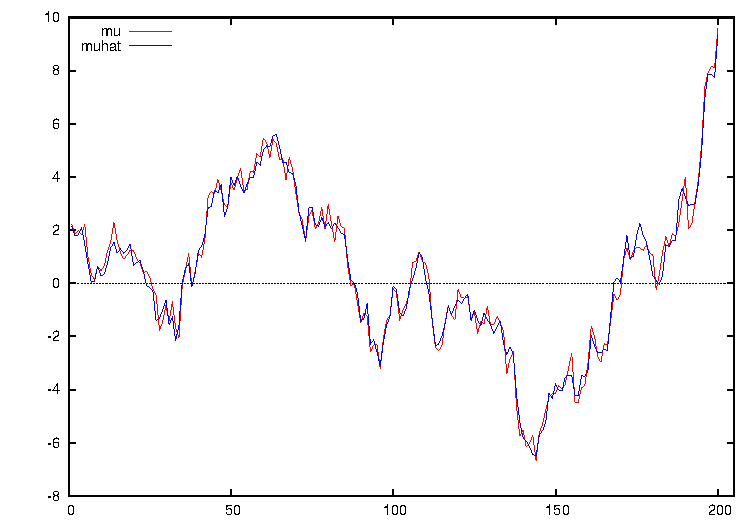
\includegraphics{figures/local_level}
  \caption{Local level model: $\mu_t$ and its smoothed estimate}
  \label{fig:loclev}
\end{figure}
By appending the following code snippet to the example in
Table~\ref{script:loclev}, one may check the results against the
\textsf{R} command \texttt{StructTS}.

\begin{code}
foreign language=R --send-data
  y <- gretldata[,"y"]
  a <- StructTS(y, type="level")
  a
  StateFromR <- as.ts(tsSmooth(a))
  gretl.export(StateFromR)
end foreign

append @dotdir/StateFromR.csv

ols Uhat 0 StateFromR --simple
\end{code}



